Para aproveitar todo o sinal fornecido pela alimentação, o retificador trifásico de onda completa utiliza uma ponte de Graetz, ou seja, de forma similar ao caso monofásico. Esse retificador aplica-se à alimentação em um arranjo $\Delta$, ou seja, sobre a tensão de linha, sem acesso ao neutro. Uma ilustração do circuito pode ser visto na figura \ref{fig:PGz}.

\begin{figure}[hb]
    \center
    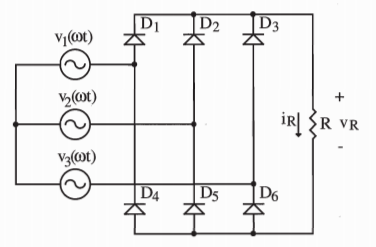
\includegraphics[scale=1.2]{imagens/PonteGraetz.PNG}
    \caption{Ponte de Graetz.}\label{fig:PGz}
    \caption*{Fonte: Eletrônica de Potência (2006)}
\end{figure}

A figura \ref{fig:FOASDRPM} mostra as formas de onda da saída.

\begin{figure}[ht]
    \center
    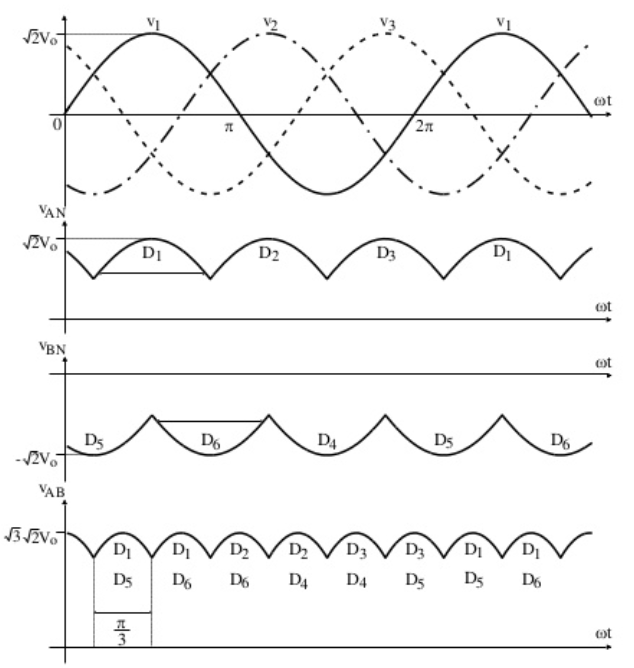
\includegraphics[scale=0.9]{imagens/FormasOndasDoisRet.PNG}
    \caption{Formas de onda da associação em série de dois retificadores de ponto médio.}\label{fig:FOASDRPM}
    \caption*{Fonte: Eletrônica de Potência (2006)}
\end{figure}

Veja que pode-se analisar a ponte de Graetz como uma associação em série de dois retificadores trifásicos de ponto médio. Além disso, vemos que os diodos entram em condução sempre em intervalos de 120 graus, logo, pela defasagem de 60 graus entre eles, sempre dois diodos estão em condução, um referente a cada semiciclo. Dessa forma, a frequência fundamental resultante é 6 vezes aquela da alimentação.

Calculando o valor médio da tensão de carga será considerado a figura .
A partir da figura \ref{fig:FOASDRPM}, podemos calcular a tensão média na carga
\begin{align*}
V_{L,med} &= \frac{3}{\pi}{\int_{-\frac{\pi}{6}}^{\frac{\pi}{6}}}{\sqrt{3}{\sqrt{2}}{V_o}}\cos(\omega{t}) \\
&= 2,34 V_o
,\end{align*} 
onde $V_o$ é o valor eficaz da tensão de alimentação.

No diodo, a corrente média \[
    I_{D,med} = \frac{I_{L,med}}{3}
\] e a corrente eficaz \[
    I_{D,ef} = \frac{I_{L,med}}{\sqrt{3}}
.\]

Um retificador trifásico com ponte de Graetz é utilizada extensivamente na indústria, onde a alimentação trifásica é mais comum, nos componentes que são projetados para utilizar corrente contínua, principalmente para altas potências (maiores que 10 KW).

